% Created 2019-06-28 Fri 15:46
% Intended LaTeX compiler: pdflatex
\documentclass[11pt]{article}
\usepackage[utf8]{inputenc}
\usepackage[T1]{fontenc}
\usepackage{graphicx}
\usepackage{grffile}
\usepackage{longtable}
\usepackage{wrapfig}
\usepackage{rotating}
\usepackage[normalem]{ulem}
\usepackage{amsmath}
\usepackage{textcomp}
\usepackage{amssymb}
\usepackage{capt-of}
\usepackage{hyperref}
\usepackage{minted}
\author{Nicolás Luarte}
\date{\today}
\title{Registro de progreso}
\hypersetup{
 pdfauthor={Nicolás Luarte},
 pdftitle={Registro de progreso},
 pdfkeywords={},
 pdfsubject={},
 pdfcreator={Emacs 25.2.2 (Org mode 9.2.3)}, 
 pdflang={English}}
\begin{document}

\maketitle
\tableofcontents

\begin{center}
\label{tab:org7508c47}
\begin{tabular}{lrrl}
Ejercicio & RPE & Peso & Fecha\\
\hline
Press banca de competencia & 7 & 92 & 11/06/2019\\
Press banca pies arriba & 7.5 & 85 & 11/06/2019\\
Press banca de competencia tempo 600 & 8 & 87.5 & 12/06/2019\\
Press banca agarre cerrado & 8 & 50 & 12/06/2019\\
Press banca de competencia & 7.5 & 95 & 14/06/2019\\
Press banca pies arriba & 8 & 87.5 & 14/06/2019\\
Press banca de competencia tempo 600 & 8 & 92.5 & 15/06/2019\\
Press banca agarre cerrado & 8 & 55 & 15/06/2019\\
Press banca de competencia & 8 & 95 & 18/06/2019\\
Press banca pies arriba & 8 & 87.5 & 18/06/2019\\
Press banca de competencia tempo 600 & 7.5 & 90 & 19/06/2019\\
Press banca agarre cerrado & 8 & 62 & 19/06/2019\\
Press banca de competencia & 8 & 95 & 21/06/2019\\
Press banca pies arriba & 8.5 & 87.5 & 21/06/2019\\
Press banca de competencia tempo 600 & 8.5 & 95 & 22/06/2019\\
Press banca agarre cerrado & 8 & 65 & 22/06/2019\\
Press banca de competencia & 8 & 100 & 24/06/2019\\
Press banca pies arriba & 8 & 90 & 24/06/2019\\
Press banca de competencia tempo 600 & 8 & 95 & 26/06/2019\\
Press banca agarre cerrado & 8 & 62.5 & 26/06/2019\\
Press banca de competencia & 8 & 97.5 & 27/06/2019\\
Press banca pies arriba & 7.5 & 90 & 27/06/2019\\
 &  &  & \\
\end{tabular}
\end{center}
\begin{center}
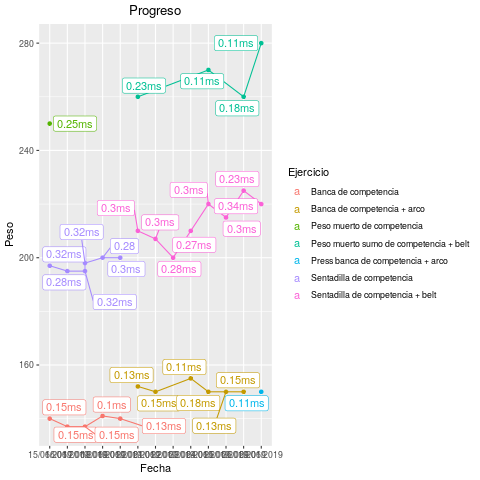
\includegraphics[width=.9\linewidth]{tmp.png}
\end{center}
\end{document}
